\documentclass{standalone}
\usepackage{tkz-fct}
\usepackage{tkz-euclide}
\usepackage{amsmath}
\usepackage{color}
\renewcommand*\familydefault{\sfdefault}
\usepackage{sansmath}
\sansmath
\definecolor{gray75}{gray}{0.75}
\begin{document}
 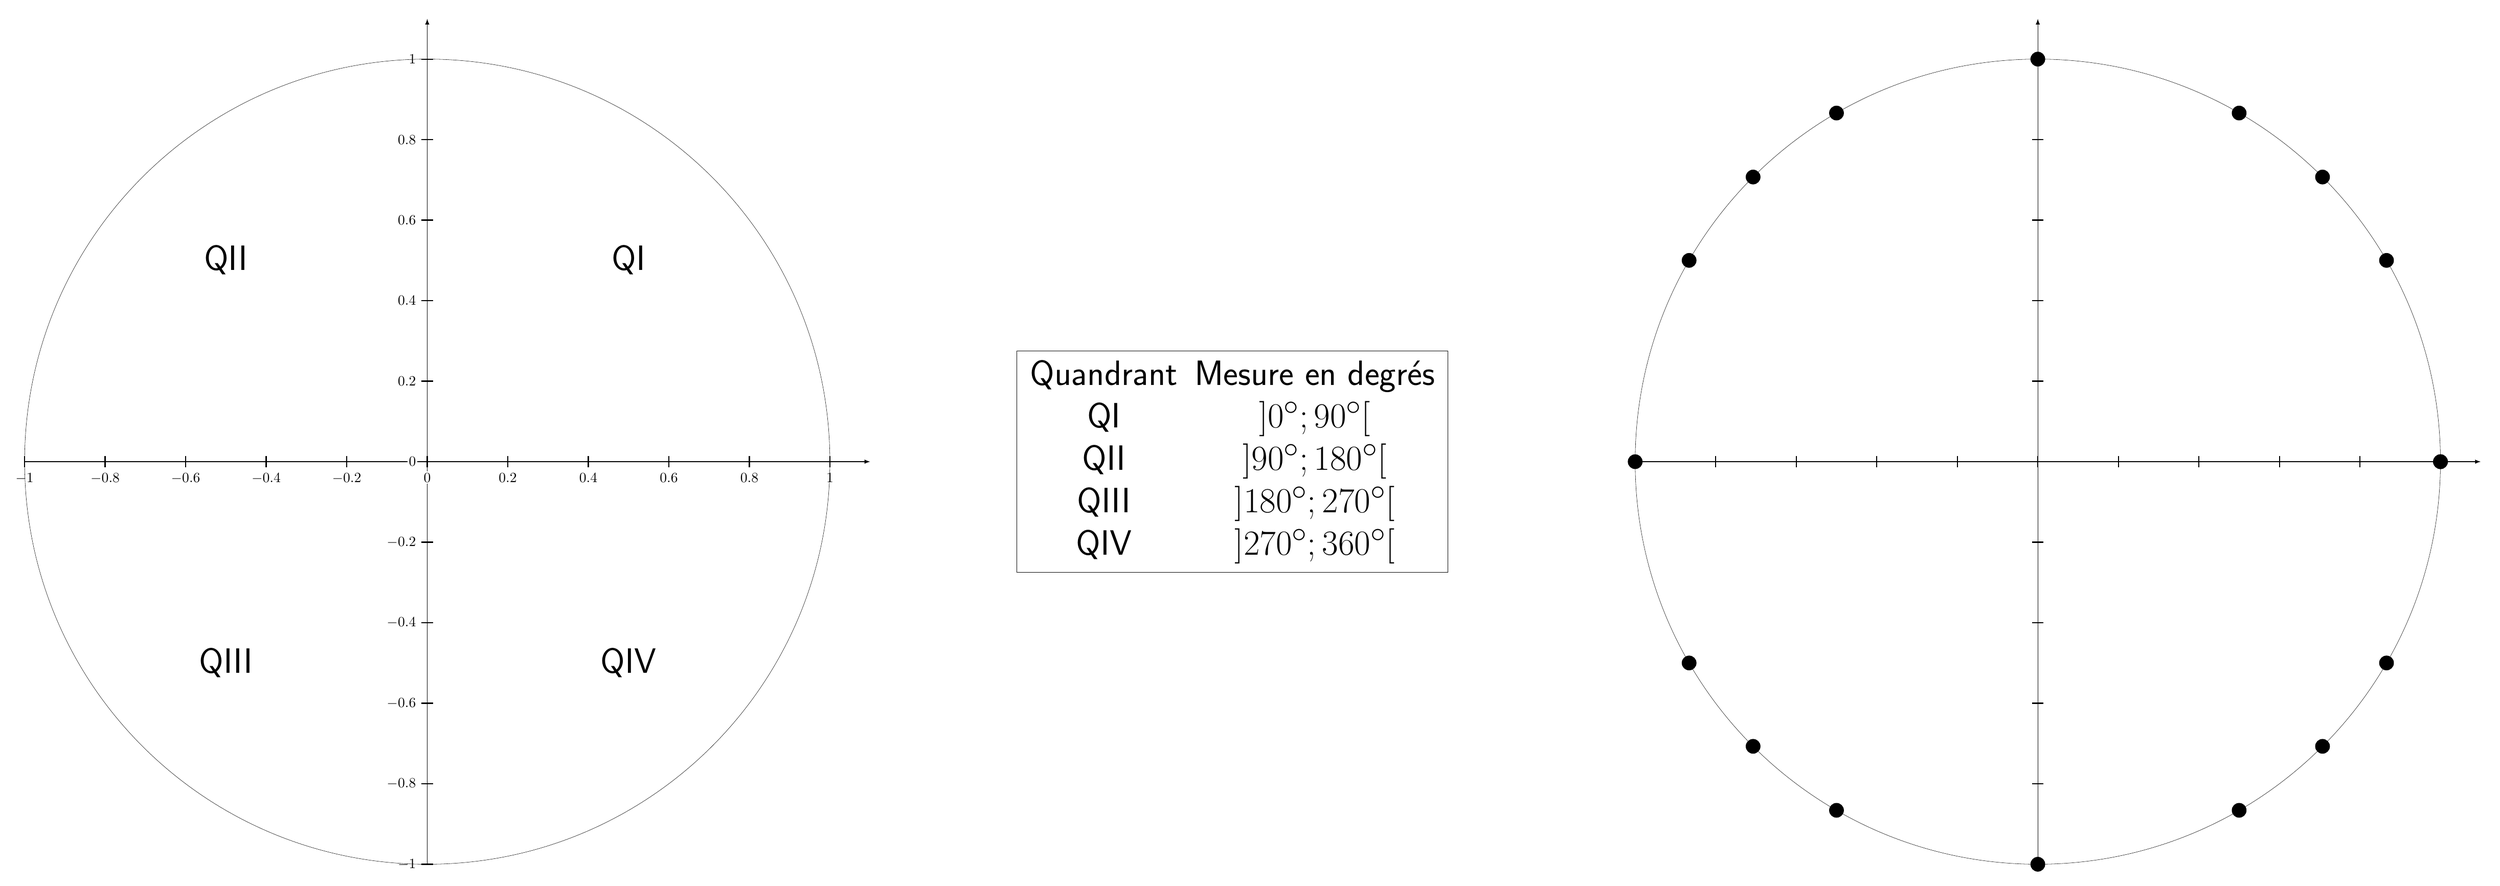
\begin{tikzpicture}[scale=2]
   \tkzInit[xmax=1.,ymax=1.,xmin=-1. ,ymin=-1,xstep=0.2,ystep=0.2]
   \tkzAxeXY[label={}]
   % \begin{scope}[dashed]
   %   \tkzGrid
   % \end{scope}

   \tkzDefPoints{0/0/O,1/0/A}
   \tkzDrawCircle[color=black](O,A)
\tkzText(.5,.5){\Huge QI}
\tkzText(-.5,.5){\Huge QII}
\tkzText(-.5,-.5){\Huge QIII}
\tkzText(.5,-.5){\Huge QIV}
\tkzText[draw](2,0){\Huge
\begin{tabular}{cc}
Quandrant & Mesure en degrés                    \\
QI        & $]0^\circ;90^\circ[$        \\
QII       & $]90^\circ;180^\circ[$    \\
QIII      & $]180^\circ;270^\circ[$   \\
QIV       & $]270^\circ;360^\circ[$ 
\end{tabular}
}
\begin{scope}[xshift=20cm]
  \tkzInit[xmax=1.,ymax=1.,xmin=-1. ,ymin=-1,xstep=0.2,ystep=0.2]
  \tkzDrawY[label={}]
%\tkzLabelY[node font=\Large]
%\tkzLabelX[node font=\Large]
\tkzDrawX[label={}]


\tkzDefPoints{0/0/O,1/0/A}

\tkzDrawCircle[color=black](O,A)
\foreach \a in {0,30,60,...,360}{%
  \tkzDefPointBy[rotation= center O angle \a](A)
  \tkzGetPoint{a}
  \tkzDrawPoint[size=10](a)
}
\foreach \a in {45,135,225,315}{%
  \tkzDefPointBy[rotation= center O angle \a](A)
  \tkzGetPoint{a}
  \tkzDrawPoint[size=10](a)
}
\end{scope}
\end{tikzpicture}
\end{document}
